\documentclass{jsarticle}
\usepackage[dvipdfmx]{graphicx}

\title{Information System Analysis 4/22日分レポート}
\author{平田 蓮 \ 6930375031}

\begin{document}
\maketitle

図~\ref{fig:lms}に、アオウミガメとアカウミガメの上腕骨の長さに対する厚みのプロットと、線形回帰の結果を示す。

\begin{figure}[h]
    \centering
    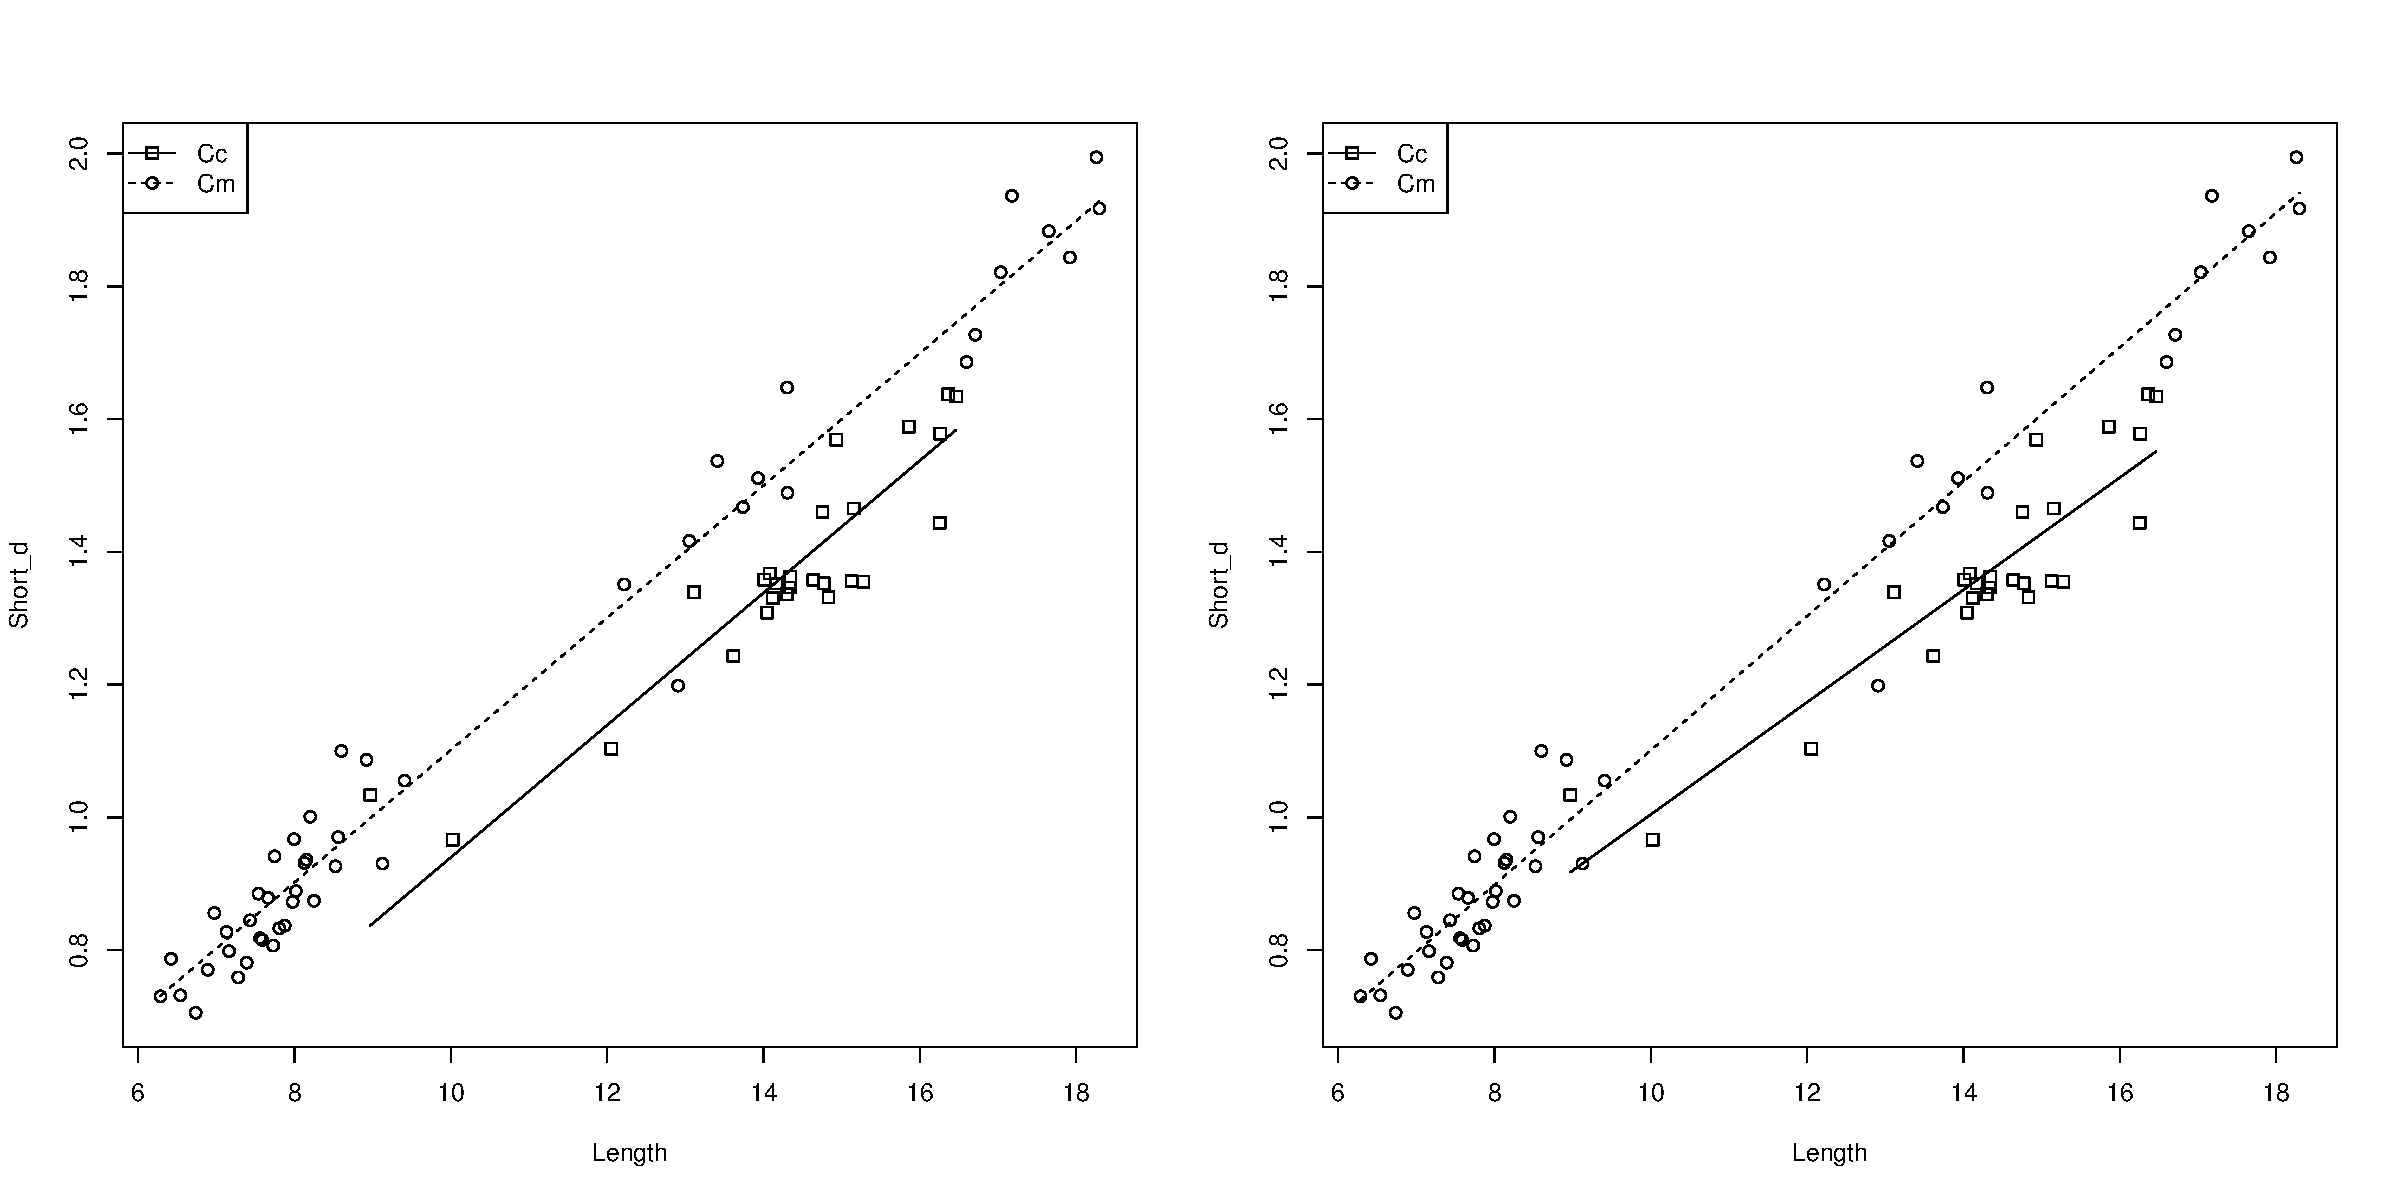
\includegraphics[width=\hsize]{lms.pdf}
    \caption{
        アオウミガメ(Cm)とアカウミガメ(Cc)の上腕骨の長さ(Length)に対する厚み(Short\_d)。
        線は交互作用を考慮していない線形モデル(左)と、交互作用を考慮している線形モデル(右)。
    }
    \label{fig:lms}
\end{figure}

\paragraph{アオウミガメ(Cm)の上腕骨の厚みが長さに対してどのように変化するかを分析しなさい。}
    アオウミガメのデータに対する線形モデルのプロットを見ると、上腕骨の厚みは長さに比例して増加することがわかる。

\paragraph{その変化はアオウミガメ(Cm)とアカウミガメ(Cc)で異なるといえるかを検証しなさい。}
    以下に、添付したRスクリプトの出力を示す。

    \begin{verbatim}
Analysis of Variance Table

Model 1: Short_d ~ Length + Species
Model 2: Short_d ~ Length * Species
  Res.Df     RSS Df Sum of Sq      F  Pr(>F)  
1     71 0.32001                              
2     70 0.30090  1   0.01911 4.4456 0.03857 *
---
Signif. codes:  0 ‘***’ 0.001 ‘**’ 0.01 ‘*’ 0.05 ‘.’ 0.1 ‘ ’ 1
       df       AIC
model1  4 -184.8141
model2  5 -187.3706
    \end{verbatim}

    この出力は、分散分析とAICの結果である。
    これらの結果より、交互作用は有意であり、交互作用を考慮したモデルの方が適切であるといえる。
    よって、上腕骨の長さに対する厚みの変化は、アオウミガメとアカウミガメで異なるといえる。

\end{document}